\documentclass[tikz]{standalone}

\usepackage{tikz}
\usetikzlibrary{shapes.arrows}

\usepackage{graphicx}

\begin{document}
    \begin{tikzpicture}
        \node (sampled_pc) {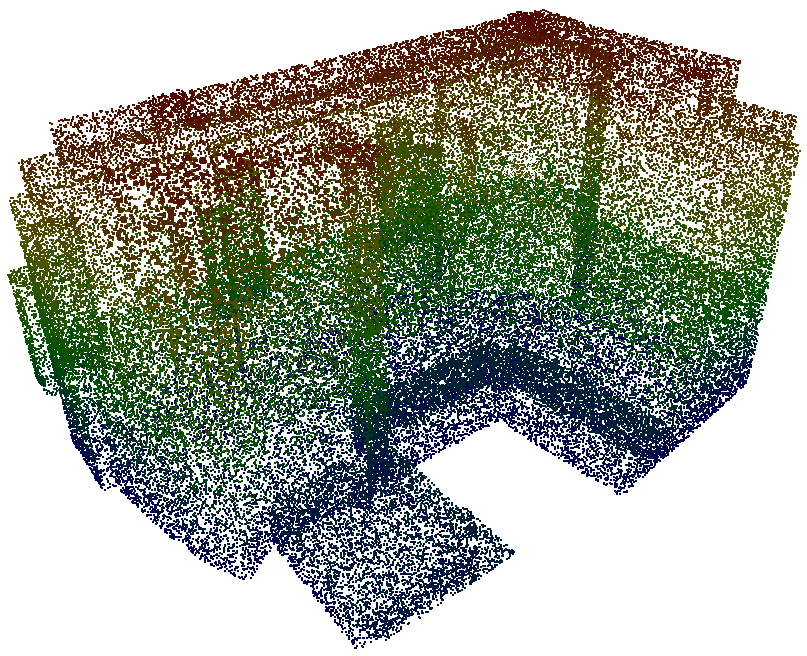
\includegraphics[width=2cm]{images/context/sampled_pc}};
        \path (sampled_pc.north) node[anchor=south, text width=5em] (sampled_pc_legend) {\scriptsize (a) Remote sensing data.};
        \path (sampled_pc.east) node[anchor=west, visible on=<2->] (3d_reconstruction) [
            draw,
            single arrow,
            color=blue,
            minimum height=1cm
        ] {3D urban modeling};
        \path (3d_reconstruction.east) node[anchor=west, visible on=<3->] (3d_model) {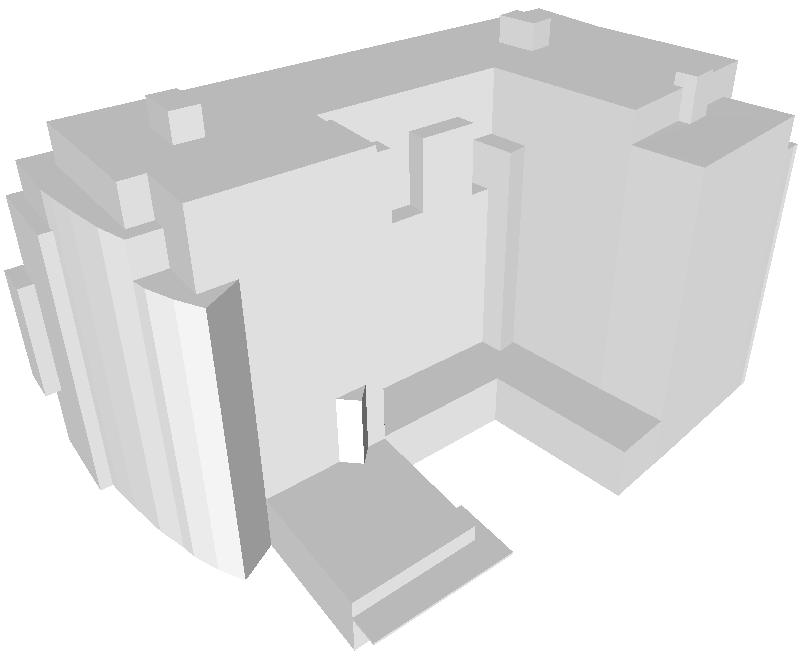
\includegraphics[width=2cm]{images/context/3d_model}};
        \path (3d_model.north) node[anchor=south, text width=6em, visible on=<3->] (3d_model_legend) {\scriptsize (b) Building model.};
        \path (3d_model.south east) node [anchor=north west, red, text width=5em, visible on=<4->] (evaluation) {How good is this model?};
        \draw[->, red, visible on=<5->] (3d_model.east) -| (evaluation.north);
    \end{tikzpicture}
\end{document}